% fig_zseq_network.tex
% TR-31: Sequence network for IBR-fed SLG fault (simplified TikZ)
%
% Three horizontal rows (pos / neg / zero sequence).
% Left: source (IBR or open).  Centre: source impedance Z_S.
% Right: line fraction alpha*Z_L.  Far right: fault terminals in series.

\begin{tikzpicture}[
  every node/.style = {font=\scriptsize},
  box/.style  = {draw=gray!60, rounded corners=3pt, fill=white,
                 inner sep=4pt, align=center, minimum width=1.6cm},
  imp/.style  = {draw=blue!60!black, fill=blue!8, rounded corners=2pt,
                 inner sep=3pt, align=center, minimum width=2.0cm,
                 minimum height=0.65cm},
  wire/.style = {thick, gray!65},
  fault/.style= {very thick, red!70!black},
]

% Row y-positions
\def\yP{0}     % positive-seq
\def\yN{-2.8}  % negative-seq
\def\yZ{-5.6}  % zero-seq

% Column x-positions
\def\xA{0}     % source
\def\xB{3.0}   % source impedance
\def\xC{6.0}   % line impedance
\def\xF{8.5}   % fault connection

% ── POSITIVE SEQUENCE ───────────────────────────────────────────────────────
\node[box, fill=green!8] at (\xA, \yP) (S1)
  {IBR\\$I_1 \leq k_\mathrm{ibr}$};
\node[imp] at (\xB, \yP) (Z1S)
  {$Z_{1S}\!=\!j0.10$};
\node[imp] at (\xC, \yP) (Z1L)
  {$\alpha Z_{1L}\!=\!j\alpha 0.05$};

\draw[wire] (S1.east)   -- (Z1S.west);
\draw[wire] (Z1S.east)  -- (Z1L.west);
\draw[wire] (Z1L.east)  -- (\xF, \yP);
% return (bottom rail)
\draw[wire] (S1.west)   -- (-0.8, \yP)
                        -- (-0.8, \yP-0.5)
                        -- (\xF+0.3, \yP-0.5) node[right,font=\tiny]{ref};

\node[blue!70!black, font=\tiny] at (4.5, \yP+0.55)
  {relay CT: $I_1$, $V_a$};

\node[font=\small, blue!80!black] at (2.5, \yP+1.2)
  {\textbf{Positive sequence}};

% ── NEGATIVE SEQUENCE ───────────────────────────────────────────────────────
\node[box, fill=green!8] at (\xA, \yN) (S2)
  {IBR\\$I_2 \!\leq\! I_1$};
\node[imp] at (\xB, \yN) (Z2S)
  {$Z_{2S}\!=\!j0.10$};
\node[imp] at (\xC, \yN) (Z2L)
  {$\alpha Z_{1L}\!=\!j\alpha 0.05$};

\draw[wire] (S2.east)   -- (Z2S.west);
\draw[wire] (Z2S.east)  -- (Z2L.west);
\draw[wire] (Z2L.east)  -- (\xF, \yN);
\draw[wire] (S2.west)   -- (-0.8, \yN)
                        -- (-0.8, \yN-0.5)
                        -- (\xF+0.3, \yN-0.5);

\node[font=\small, orange!70!black] at (2.5, \yN+1.2)
  {\textbf{Negative sequence}};

% Delta-transformer note
\node[draw=orange!60, fill=orange!8, rounded corners=2pt,
      font=\tiny, inner sep=2pt, align=center]
  at (-1.2, -1.4)
  {$\Delta$ winding:\\blocks $I_0$};

% ── ZERO SEQUENCE ───────────────────────────────────────────────────────────
\node[draw=red!60, fill=red!8, rounded corners=3pt,
      inner sep=4pt, align=center] at (\xA, \yZ) (S0)
  {OPEN\\$\Delta$ xfmr\\$I_0^{IBR}\!=\!0$};
\node[imp] at (\xB, \yZ) (Z0S)
  {$Z_{0S}\!=\!j0.30$\\{\tiny(network earthing)}};
\node[imp] at (\xC, \yZ) (Z0L)
  {$\alpha Z_{0L}\!=\!j\alpha 0.15$};

% dashed "open" connection from S0
\draw[wire, red!60, dashed] (S0.east) -- (1.5, \yZ)
  node[above, font=\tiny, red!60]{no path};
% solid from Z0S
\draw[wire] (1.5, \yZ) -- (Z0S.west);
\draw[wire] (Z0S.east)  -- (Z0L.west);
\draw[wire] (Z0L.east)  -- (\xF, \yZ);
\draw[wire] (1.5, \yZ)  -- (1.5, \yZ-0.5)
                        -- (\xF+0.3, \yZ-0.5) node[right,font=\tiny]{earth};

% I0 flow arrow
\draw[->, very thick, red!50!black]
  (3.8, \yZ+0.40) -- (5.4, \yZ+0.40);
\node[red!60!black, font=\tiny, above] at (4.6, \yZ+0.40)
  {$I_0$ (network, indep.\ of $k_\mathrm{ibr}$)};

\node[font=\small, red!70!black] at (2.5, \yZ+1.2)
  {\textbf{Zero sequence: $I_0$ from network earthing}};

% ── FAULT SERIES CONNECTION ─────────────────────────────────────────────────
\node[draw=red!70, fill=red!15, rounded corners=3pt,
      inner sep=4pt, align=center, font=\small]
  at (\xF+1.2, \yN) (FP)
  {\textbf{Fault}\\$V_a\!=\!0$};

\draw[fault, ->] (\xF, \yP)   -- (FP.north);
\draw[fault]     (\xF, \yN)   -- (FP.west);
\draw[fault, ->] (\xF, \yZ)   -- (FP.south);

% boundary conditions
\node[draw=gray!50, fill=yellow!8, rounded corners=2pt,
      font=\tiny, inner sep=3pt, align=left]
  at (\xF+2.8, \yN)
  {SLG BC at fault:\\
   $V_a = 0$,\; $I_b=I_c=0$\\
   $\Rightarrow I_1\!=\!I_2\!=\!I_0$\\
   but $|I_1| \ll |I_0|$ for IBR};

% ── KEY RESULT BOX ──────────────────────────────────────────────────────────
\node[draw=blue!50, fill=blue!5, rounded corners=4pt,
      font=\small, inner sep=6pt, align=left]
  at (4.5, -7.6)
  {$k_0 = \dfrac{Z_{0L}-Z_{1L}}{3Z_{1L}}
       = \dfrac{0.15-0.05}{0.15} = 0.667$
   \quad (line parameter, source-independent)\\[4pt]
   BUT: $|I_0| \approx 1.8$\,pu $\gg |I_1| = k_\mathrm{ibr} \leq 0.20$\,pu
   $\;\Rightarrow\;$ relay over-estimates $Z_m$ by $3$--$8\times$};

\end{tikzpicture}
